
\chapter{Algoritmo memético para el MC-TTRP}\label{chapter:3}
En este capítulo se tratará el algoritmo memético ideado para dar solución al problema MC-TTRP planteado en el Capítulo \ref{chapter:2}. En primer lugar, se hará una introducción al método mediante una explicación del trabajo relacionado ya existente sobre este problema y otros problemas similares. En segundo lugar se mostrará el algoritmo, el cual será ilustrado mediante ejemplos visuales de los métodos utilizados como operadores del algoritmo genético. Finalmente, se explicarán las pruebas realizadas para mostrar el funcionamiento del algoritmo creado.

\section{Trabajo relacionado}\label{section:trabajo-rel}
Como se indica en el Capítulo \ref{chapter:2}, el problema del MC-TTRP nace de la unión de otros dos problemas de rutas, el problema de rutas multicompartimento (MC-VRP) y el problema de rutas de tráileres y camiones (TTRP). Ambos problemas han sido tratados anteriormente por otros autores y se han ofrecido soluciones basadas en múltiples heurísticas o metaheurísticas, destacando los resultados obtenidos mediante métodos tabú \cite{chao-ttrp,laura-mcttrp}. Sin embargo, los métodos tabú no son los únicos que han obtenido buenos resultados para los problemas de rutas. Los algoritmos genéticos o meméticos han obtenido muy buenos resultados para diversas modificaciones de los problemas de rutas (\cite{thangiah-1995} para el VRPTW, o \cite{prins-2003} para un VRP genérico).\\

Ambos problemas que componen el MC-TTRP han sido abordados de manera satisfactoria en la literatura mediante el uso de algoritmos evolutivos. El uso de algoritmos meméticos destaca sobre todo en el caso de los problemas de rutas con vehículos multicompartimento. En \cite{MC-VRP-Memetic-ElFallahi}, se define un algoritmo memético y se compara con un método tabú. En esta comparación, el algoritmo de búsqueda tabú obtiene mejores resultados, sin embargo, el tiempo utilizado en la ejecución es menor para el algoritmo memético. También se ha investigado el uso de algoritmos meméticos en variaciones del MC-VRP. Por ejemplo, en \cite{MC-VRP-Stochastic-Mendoza}, se estudia el uso de un algoritmo memético para la resolución de un problema de rutas con vehículos multicompartimento con demandas estocásticas. Para el TTRP, los algoritmos basados en búsquedas tabú o búsquedas locales son mayoritarios. No obstante, si que ha existido algún interés por la utilización de algoritmos genéticos o meméticos para la resolución de este problema, como puede verse en \cite{ttrp-memetic}. En este artículo se muestran mejoras del algoritmo memético con respecto a otros similares para resolver el problema del TTRP.\\

Finalmente, para el problema del MC-TTRP, no se identificaron, durante la revisión realizada, algoritmos meméticos o genéticos previamente reportados en la literatura. Por lo tanto, el algoritmo propuesto puede considerarse una primera aproximación a su resolución mediante este tipo de metaheurísticas. Para idear este algoritmo se han utilizado como base distintos artículos, pero principalmente se destacan \cite{MC-VRP-Memetic-ElFallahi,MC-VRP-Stochastic-Mendoza,laura-mcttrp}. Los dos primeros artículos tratan el MC-VRP desde una perspectiva memética, dando un posible esqueleto del algoritmo, además de indicar posibles métodos de optimización locales. El último artículo explica la resolución del MC-TTRP mediante otras metaheurísticas distintas, ofreciendo posibles alternativas para afrontar las restricciones que añade este problema sobre el MC-VRP. 

\section{Algoritmo memético}\label{section:MA}
Veamos ahora el algoritmo memético ideado para solucionar el MC-TTRP.
\subsection{Consideraciones previas} \label{section:cons-tom}
Aunque se ha intentado seguir lo más cerca posible tanto la descripción del problema, como el modelo PLEM dados en el Capítulo \ref{chapter:2}, se ha tenido en cuenta alguna consideración que no se contempla en este modelo.\\

Se ha requerido que las subrutas que comienzan en un cliente VC en una ruta mixta, solo puedan estar formadas por clientes TC. Es decir, los clientes VC sólo podrán ser servidos por un vehículo completo en una ruta de tráiler o por un camión en una ruta de camión. Esta restricción ha sido añadida para conseguir una simplificación de la programación, sobre todo en la codificación de las soluciones como cromosomas de un modelo memético. A causa de esta restricción, los resultados del algoritmo serán, por lo general, peores que aquellos métodos con los que este será comparado. Además, por temas de logística, el camión y el tráiler no pueden ser separados durante el abastecimiento, por lo que no se pueden almacenar los bienes para clientes VC en el camión. Por lo demás, todas las restricciones tratadas en el capítulo anterior se tendrán en cuenta para obtener la mejor solución posible. Es destacable que las condiciones \eqref{eq-mcttrp:2.3} y \eqref{eq-mcttrp:2.6} se tienen en cuenta, por lo que un cliente deberá ser completamente abastecido por un único vehículo (ya sea un camión o un vehículo completo). Esto es distinto a lo que otros algoritmos de resolución del MC-VRP utilizan, por lo que no serán comparables. 

\subsection{Esquema general del algoritmo}
Veamos en primer lugar el esquema del algoritmo. Como se indica en la Sección \ref{section:trabajo-rel}, los principales algoritmos meméticos en los que nos basaremos son aquellos dados en \cite{MC-VRP-Memetic-ElFallahi,MC-VRP-Stochastic-Mendoza}.\\
\subsubsection{Población inicial y finalización}

El algoritmo comienza definiendo una población inicial de tamaño $N$ que se denominará $\mathscr{P}_0$. Esta población puede ser elegida mediante múltiples métodos. Un ejemplo se da en \cite{ttrp-memetic} o en \cite{MC-VRP-Memetic-ElFallahi}. En ambos artículos, $\mathscr{P}_0$ es la combinación de un conjunto de individuos generados de manera aleatoria y un conjunto de buenas soluciones generado a partir de algún tipo de heurística. En el primer artículo, por ejemplo, la heurística utilizada es la denominada como heurística de ahorros de Clarke y Wright \cite{clarke-1964}. Esta es una de las heurísticas más comunes para la resolución del TSP. En \cite{laura-mcttrp} se desarrolla un método para aplicar esta heurística al MC-TTRP, sin embargo, en mi caso he optado por comenzar en una población inicial completamente aleatoria. Esto se debe a varios motivos. En primer lugar, en los artículos anteriormente tratados, se puede observar que la mejora obtenida por comenzar con una población alimentada con resultados provenientes de alguna heurística no es significativa. En segundo lugar, la extensión de la heurística CW al MC-TTRP es bastante compleja y el tiempo de ejecución del algoritmo memético es bajo, por lo que puede aumentar mucho el tiempo de ejecución del algoritmo.\\

Además de $\mathscr{P}_0$, también se definen 2 parámetros, $\alpha$ y $\beta$ ($\beta\leq\alpha$). Estos parámetros serán los encargados de finalizar la optimización. El motivo de la existencia de dos parámetros es que miden distintos criterios de finalización. La función de $\alpha$ es medir el número total de iteraciones ($max_{iter}$) realizadas por el método, mientras que $\beta$ almacena el número de iteraciones seguidas en las cuales no se ha mejorado el óptimo ($max_{nopt}$). Es decir, en general, nuestro criterio de finalización será que se haya cumplido un número total de iteraciones o que la población haya sido lo suficientemente explorada (no se generan mejores resultados en un cierto número de iteraciones).\\

Una vez explicada la inicialización y la finalización del método, veamos el esquema principal del método. En este esquema se considera que $\mathscr{P}_\alpha$ hace referencia a la población en la iteración $\alpha$ de la optimización. Además de la población $\mathscr{P}$, se deberá considerar la población extendida en la iteración $\alpha$ o $\mathscr{E}_\alpha$. La población extendida puede verse como la población del paso $\alpha$ a la cual se le añaden los nuevos individuos generados por los distintos operadores del algoritmo memético. Esta población extendida será acotada para obtener $\mathscr{P}_{\alpha+1}$. En este método también aparecen reflejadas 3 probabilidades: $p_c$, $p_m$ y $p_{ls}$. Estas probabilidades son parámetros del problema y definen la probabilidad de efectuar el cruce, la mutación y la búsqueda local respectivamente. $p_c$ tiene más complejidad ya que sirve para obtener el número de individuos generados por cruce, es decir, representa el porcentaje del tamaño de la población que será generado mediante cruce. Además, la función objetivo será denominada $f$. Una vez explicados todos los parámetros, en el Algoritmo \ref{alg:MA-skeleton} se muestran los pasos seguidos para obtener el valor mínimo de la solución del MC-TTRP mediante un algoritmo memético.

\begin{algorithm}[!t]
    \caption{Algoritmo memético para el MC-TTRP}
    \label{alg:MA-skeleton}
    \begin{algorithmic}[1]
        \State \textbf{Inicialización:}
        \State Selección de $\mathscr{P}_0$
        \State $\alpha\leftarrow0;\;\beta\leftarrow 0;\;min_{cost}\leftarrow+\infty$
        \State \textbf{Optimización:}
        \While {$\alpha<max_{iter},\;\beta<max_{nopt}$}
            \State $\mathscr{E}_\alpha\leftarrow\mathscr{P}_\alpha$
            \State $nCruce\leftarrow \lceil p_c*|\mathscr{P}_\alpha|\rceil$
            \While{$nCruce>0$}
                \State Selección de 2 padres
                \State Generación del hijo $c$ mediante cruce
                \State Evaluación y reparación de $c$
                \State Introducción de $c$ en $\mathscr{E}_\alpha$
                \State $nCruce \leftarrow nCruce -1$
            \EndWhile
            \For {cada individuo $s\in\mathscr{P}_\alpha$}
                \State Mutación de $s$ con probabilidad $p_m$ para generar $s'$
                \State Evaluación e introducción de $s'$ en $\mathscr{E}_{\alpha}$
                \State Aplicación del método de búsqueda local a $s$ con probabilidad $p_{ls}$ para generar $s''$
                \State Evaluación e introducción de $s''$ en $\mathscr{E}_{\alpha}$
            \EndFor
            \State Selección de los $N$ mejores individuos en $\mathscr{E}_\alpha$ para formar $\mathscr{P}_{\alpha+1}$
            \If {$\min_{x\in\mathscr{P}_{\alpha+1}}f(x)<min_{cost}$}
                \State $min_{cost}\leftarrow\min_{x\in\mathscr{P}_{\alpha+1}}f(x)$
                \State $\beta\leftarrow 0$
            \Else
                \State $\beta\leftarrow\beta+1$
            \EndIf
            \State $\alpha\leftarrow\alpha+1$
        \EndWhile
    \end{algorithmic}
\end{algorithm}

\subsection{Codificación de los cromosomas}
Una vez tratada la estructura básica del algoritmo, veamos como funciona cada una de las operaciones que lo conforman. Sin embargo, antes de comenzar, será necesario tratar la manera en la que se codifican los cromosomas del algoritmo memético.\\

En primer lugar, los cromosomas de este método representan la solución que representa cada individuo, es decir, el conjunto de rutas tomado y el tipo de cada ruta. Esta representación deberá estar definida de una manera eficiente y que permita el uso del resto de los operadores del método. Para ello se ha utilizado una codificación específica para los problemas de rutas, la denominada GVR \cite{gvr}. Esta codificación sustituye a la codificación clásica de los cromosomas de los algoritmos genéticos para los problemas de rutas, que consistía en una permutación de los nodos del grafo con $0$ ficticios para marcar el fin de las rutas. Con la codificación clásica, los métodos de cruce y mutación tenían que ser específicos, ya que había que tener en cuenta la existencia de los delimitadores. Para evitar esto, nace la codificación GVR. Esta representación ve los cromosomas como un conjunto de vectores (desde un punto de vista informático) que representa cada una de las rutas de la solución (se puede ver un ejemplo en la Figura \ref{fig:GVR_crom}). Esta codificación permite la utilización de métodos de cruce, mutación y de búsqueda local eficientes y efectivos. \\

No obstante no se ha respondido a la otra pregunta, ¿cómo se puede saber el tipo de ruta que representa cada vector del cromosoma? La respuesta es sencilla, ya que para cualquier ruta de un problema MC-TTRP, el tipo de ruta está completamente definido por el tipo de cliente que sea el primer individuo de la ruta. Es decir, en el caso de que el primer cliente sea un VC, la ruta será o mixta o una ruta de vehículos, mientras que si el primer cliente es un cliente TC, la ruta será de camión. Esto se debe a que en cualquiera de estas rutas se permite la existencia de ambos clientes, como se puede ver en la Figura \ref{fig:TTRP}. Para identificar las subrutas, sin embargo, el proceso no es tan sencillo, y es por esto por lo que se ha añadido la restricción comentada en la Sección \ref{section:cons-tom}. Las subrutas estarán formadas, en esta codificación, por aquellos clientes del tipo TC que se encuentren dentro de una ruta de tráiler. De esta manera, con esta codificación tan sencilla, será posible representar todas las posibles configuraciones de rutas factibles, y, por consiguiente, ejecutar el algoritmo memético. Veamos como se utilizan los cromosomas GVR para realizar las operaciones definidas por el algoritmo.

\begin{figure}[t]
    \centering
    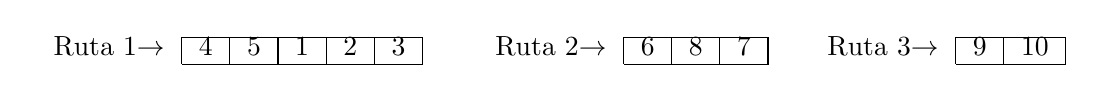
\begin{tikzpicture}
        \node (padres) at (0,0) {\begin{tabular}{l|c |c |c |c |c |}
            \cline{2-6}
            Ruta 1$\rightarrow$ & $4$ & $5$ & $1$ & $2$ & $3$ \\ \cline{2-6} 
            \end{tabular}};
        \node (hijos) at (5,0) {\begin{tabular}{l|c |c |c |}
            \cline{2-4}
            Ruta 2$\rightarrow$ & $6$ & $8$ & $7$ \\ \cline{2-4} 
            \end{tabular}};
        \node at (9,0) {\begin{tabular}{l|c |c |}
            \cline{2-3}
            Ruta 3$\rightarrow$ & $9$ & $10$\\ \cline{2-3} 
            \end{tabular}};
    \end{tikzpicture}
    \caption{Ejemplo de un cromosoma GVR para un problema con 10 nodos.}
    \label{fig:GVR_crom}
\end{figure}

\subsection{Cruce}
En primer lugar, describiremos el algoritmo de cruce utilizado. Este algoritmo es el cruce básico a partir de los cromosomas GVR y se define en \cite{gvr}. Según el artículo, este cruce debería realizarse sobre cada elemento de la población, eligiendo el segundo padre de manera aleatoria. Sin embargo, nosotros hemos escogido realizar una selección por torneo entre 4 padres aleatorios de la población para cada cruce. Esta elección se debe a la naturaleza del Algoritmo \ref{alg:MA-skeleton}, que utiliza una probabilidad $p_c$ para elegir el número de cruces que se realizarán para obtener nuevos cromosomas. Una vez elegidos los padres a cruzar, los pasos del algoritmo son los siguientes:
\begin{enumerate}
    \item Selección de uno de los padres como el receptor y otro como el emisor. En nuestro caso, el primer padre elegido por torneo será el receptor y el segundo el emisor.
    \item Selección de una subruta $S=\{a_1,\ldots,a_n\}$ de una de las rutas del padre emisor. Esta subruta puede ser de cualquier tamaño, desde la ruta entera hasta un solo elemento (en este último caso, el cruce podría ser visto como una relocalización).
    \item Búsqueda del elemento $b$ del padre receptor tal que el camino de $b$ a $a_1$ sea el menor posible.
    \item Introducción de la subruta $S$ tras el elemento $b$ para formar el hijo $c$.
    \item Eliminación de los elementos duplicados en el hijo. Es decir, se reorganizan las rutas para que los elementos añadidos por la subruta sean únicos.
\end{enumerate}

En la Figura \ref{fig:crossoverGVR} puede verse gráficamente el funcionamiento de este algoritmo.

\begin{figure}[t]
    \centering
    \resizebox{\textwidth}{!}{%
    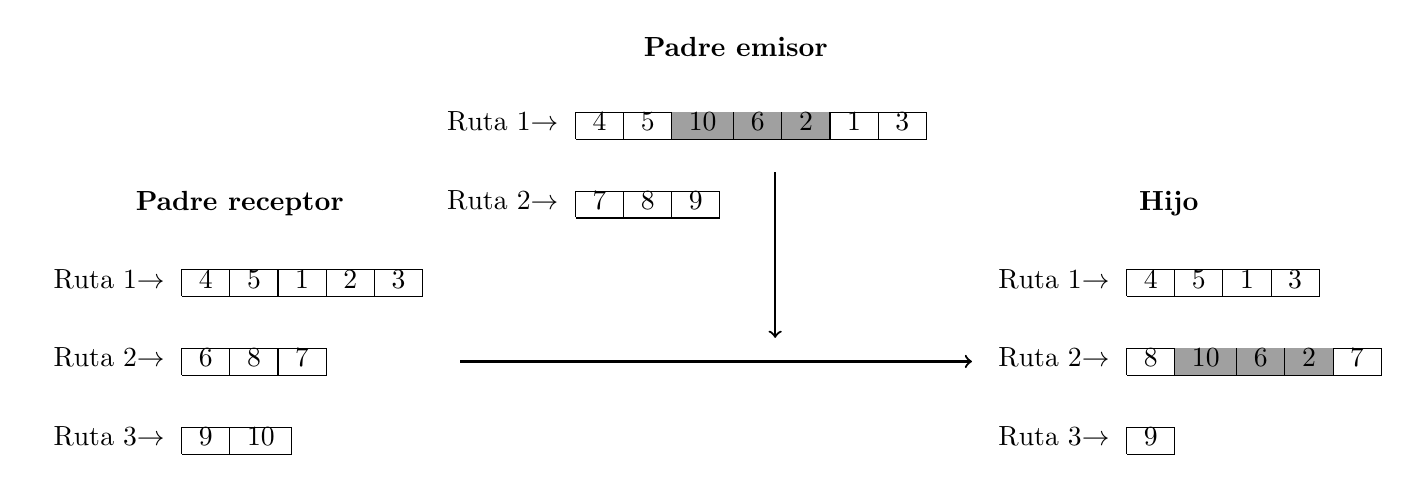
\begin{tikzpicture}
        % Padre 1
        \node (padre1) at (2.7,1) {\textbf{Padre receptor}};
        \node[anchor=west] (padre1r1) at (0,0) {\begin{tabular}{l|c |c |c |c |c |}
            \cline{2-6}
            Ruta 1$\rightarrow$ & $4$ & $5$ & $1$ & $2$ & $3$ \\ \cline{2-6} 
            \end{tabular}};
        \node[anchor=west] (padre1r2) at (0,-1) {\begin{tabular}{l|c |c |c |}
            \cline{2-4}
            Ruta 2$\rightarrow$ & $6$ & $8$ & $7$ \\ \cline{2-4} 
            \end{tabular}};
        \node[anchor=west] (padre1r3) at (0,-2) {\begin{tabular}{l|c |c |}
            \cline{2-3}
            Ruta 3$\rightarrow$ & $9$ & $10$\\ \cline{2-3} 
            \end{tabular}};

        % Padre 2
        \node (padre2) at (9,3) {\textbf{Padre emisor}};
        \node[anchor=west] (padre2r1) at (5,2) {\begin{tabular}{l|c |c | >{\columncolor[HTML]{A0A0A0}}c |>{\columncolor[HTML]{A0A0A0}}c |>{\columncolor[HTML]{A0A0A0}}c | c | c |}
            \cline{2-8}
            Ruta 1$\rightarrow$ & $4$ & $5$ & $10$ & $6$ & $2$ & $1$ & $3$\\ \cline{2-8}
            \end{tabular}};
        \node[anchor=west] (padre2r2) at (5,1) {\begin{tabular}{l|c |c |c |}
            \cline{2-4}
            Ruta 2$\rightarrow$ & $7$ & $8$ & $9$ \\ \cline{2-4} 
            \end{tabular}};
    
        % Hijo
        \node (hijo) at (14.5,1) {\textbf{Hijo}};
        \node[anchor=west] (hijor1) at (12,0) {\begin{tabular}{l|c |c |c |c |}
            \cline{2-5}
            Ruta 1$\rightarrow$ & $4$ & $5$ & $1$ & $3$ \\ \cline{2-5} 
            \end{tabular}};
        \node[anchor=west] (hijor2) at (12,-1) {\begin{tabular}{l|c |>{\columncolor[HTML]{A0A0A0}}c |>{\columncolor[HTML]{A0A0A0}}c |>{\columncolor[HTML]{A0A0A0}}c |c |}
            \cline{2-6}
            Ruta 2$\rightarrow$ & $8$ & $10$ & $6$ & $2$ & $7$ \\ \cline{2-6} 
            \end{tabular}};
        \node[anchor=west] (hijor3) at (12,-2) {\begin{tabular}{l|c|}
            \cline{2-2}
            Ruta 3$\rightarrow$ & $9$ \\ \cline{2-2} 
            \end{tabular}};

        \draw[thick,-to] (5.5,-1) -- (hijor2);
        \draw[thick,-to] (9.5,1.4) -- (9.5,-0.7);
            
    \end{tikzpicture}
    }%
    \caption{Crossover para GVR.}
    \label{fig:crossoverGVR}
\end{figure}

\subsection{Mutación}
Una vez realizado el cruce, se podrá ejecutar la mutación sobre los elementos de la población. Si seguimos el Algoritmo \ref{alg:MA-skeleton}, podemos ver que la mutación se ejecuta sobre los elementos de la población $\mathscr{P}_\alpha$, que no incluye aquellos elementos generados por cruce. Esto da igual, ya que los elementos de la población son generados de manera independiente, y aquellos individuos generados por cruce, estarán en la siguiente población. Para la mutación, \cite{gvr} ofrece múltiples métodos, como pueden ser el intercambio, la inversión, la inserción y el desplazamiento. En nuestro caso, debido a que nuestro algoritmo se basa en \cite{MC-VRP-Stochastic-Mendoza}, utilizaremos la misma mutación que se utiliza en este artículo, la inversión de subrutas. Cabe destacar que una modificación de la inserción será utilizada en un futuro como parte de los métodos de búsqueda local.\\

La inversión de rutas es una de las maneras más directas de mutar los cromosomas GVR, ya que se introducen variaciones en la población realizando en esencia, permutaciones de los elementos, como se trataba en la Sección \ref{section:mutacion-genetic}. De esta manera, la mutación funcionará mediante la elección de una subruta aleatoria en el individuo e invirtiendo los elementos de la ruta. En la Figura \ref{fig:mutacion-GVR} se puede ver como funcionaría esta mutación sobre un posible cromosoma GVR.

\begin{figure}[b]
    \centering
    \resizebox{0.75\textwidth}{!}{%
    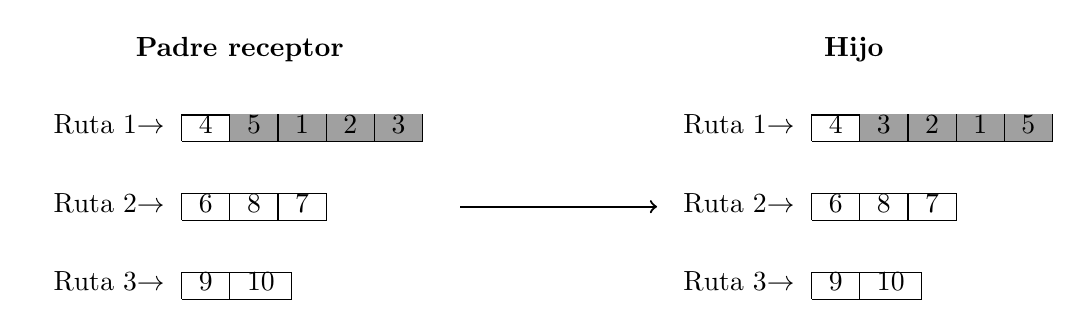
\begin{tikzpicture}
        % Padre 1
        \node (padre1) at (2.7,1) {\textbf{Padre receptor}};
        \node[anchor=west] (padre1r1) at (0,0) {\begin{tabular}{l|c |>{\columncolor[HTML]{A0A0A0}}c |>{\columncolor[HTML]{A0A0A0}}c |>{\columncolor[HTML]{A0A0A0}}c |>{\columncolor[HTML]{A0A0A0}}c |}
            \cline{2-6}
            Ruta 1$\rightarrow$ & $4$ & $5$ & $1$ & $2$ & $3$ \\ \cline{2-6} 
            \end{tabular}};
        \node[anchor=west] (padre1r2) at (0,-1) {\begin{tabular}{l|c |c |c |}
            \cline{2-4}
            Ruta 2$\rightarrow$ & $6$ & $8$ & $7$ \\ \cline{2-4} 
            \end{tabular}};
        \node[anchor=west] (padre1r3) at (0,-2) {\begin{tabular}{l|c |c |}
            \cline{2-3}
            Ruta 3$\rightarrow$ & $9$ & $10$\\ \cline{2-3} 
            \end{tabular}};
            
        % Hijo
        \node (hijo) at (10.5,1) {\textbf{Hijo}};
        \node[anchor=west] (hijor1) at (8,0) {\begin{tabular}{l|c |>{\columncolor[HTML]{A0A0A0}}c |>{\columncolor[HTML]{A0A0A0}}c |>{\columncolor[HTML]{A0A0A0}}c |>{\columncolor[HTML]{A0A0A0}}c |}
            \cline{2-6}
            Ruta 1$\rightarrow$ & $4$ & $3$ & $2$ & $1$ & $5$ \\ \cline{2-6}
            \end{tabular}};
        \node[anchor=west] (hijor2) at (8,-1) {\begin{tabular}{l|c |c |c |}
            \cline{2-4}
            Ruta 2$\rightarrow$ & $6$ & $8$ & $7$ \\ \cline{2-4}
            \end{tabular}};
        \node[anchor=west] (hijor3) at (8,-2) {\begin{tabular}{l|c| c|}
            \cline{2-3}
            Ruta 3$\rightarrow$ & $9$ & $10$\\ \cline{2-3} 
            \end{tabular}};

        \draw[thick,-to] (5.5,-1) -- (hijor2);
    \end{tikzpicture}
    }%
    \caption{Mutación de inversión de rutas para GVR.}
    \label{fig:mutacion-GVR}
\end{figure}
\subsection{Búsquedas locales}
Una vez tratados los métodos básicos de los algoritmos genéticos, veamos aquellos operadores que convierten un algoritmo genético en uno memético, los métodos de búsquedas locales. El método utilizado de búsqueda local utiliza la combinación de dos operadores, aunque podrían añadirse más operadores. Estos operadores locales están basados en el método de búsqueda local utilizado en \cite{MC-VRP-Stochastic-Mendoza}, que combina la relocalización y el método 2-OPT para recorrer el vecindario de soluciones. Veamos como funcionan estos métodos de optimización de manera independiente y cómo estos pueden ser combinados de manera eficiente.
\begin{itemize}
    \bditem{Relocalización: }La relocalización trata de mover un nodo a otra ruta de tal manera que se mejore la solución original. Nuestro método solo permite relocalizaciones que mejoren la solución original. Si ningún movimiento mejora la solución, no se realiza ninguna operación.
    \bditem{2-OPT:} Este método es un método de optimización local ideado para solucionar el problema del TSP \cite{croes-1958}. La idea detrás de este método es la eliminación de los cruces dentro de una ruta. Para ello, se seleccionan 2 ejes de una ruta y se invierten los nodos que existen entre esos ejes. De esta manera, en caso de que existiese un cruce sobre el grafo, este sería eliminado, dando lugar a un camino más corto. Este método, como se puede ver, solo se puede utilizar para modificar una única ruta del cromosoma. 
\end{itemize}
Como se había indicado, nuestro método de búsqueda local combinará los dos métodos de búsqueda locales anteriores. En primer lugar, se realizará la relocalización hasta que se encuentre un movimiento que mejora la solución. Una vez realizada la relocalización, se utilizará 2-OPT sobre la ruta en la que se ha añadido un nuevo elemento. De esta manera, se podrá buscar una configuración de elementos que minimice el coste de esa ruta. Cabe destacar que el procedimiento 2-OPT adquiere una relevancia particular en la resolución del MC-TTRP, especialmente debido a la restricción adicional descrita en la Sección \ref{section:cons-tom}. Al reorganizar la ruta, se penalizará la separación de subrutas y se premiará la unión de los clientes TC, obteniendo subrutas de mayor tamaño. En la Figura \ref{fig:busq-local} se puede observar un ejemplo de la modificación de las rutas realizadas por el método de búsqueda local.
\begin{figure}[!t]
    \centering
    \resizebox{\textwidth}{!}{%
    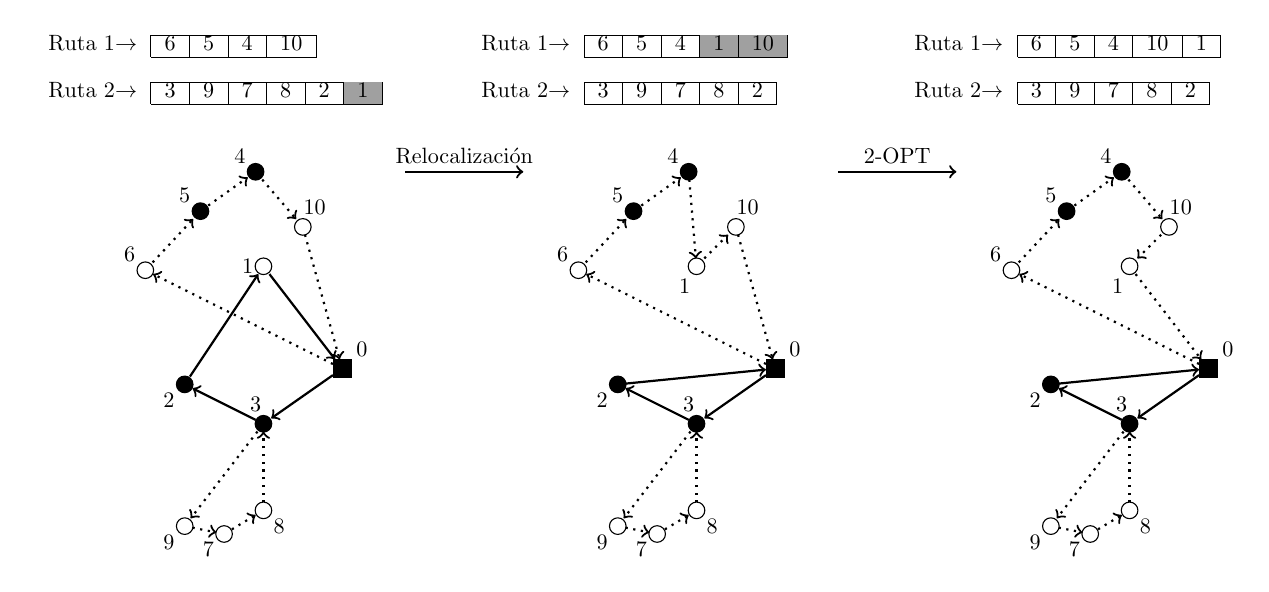
\begin{tikzpicture}[scale=1, every node/.style={scale=0.8}]
    
      % Depot
      \node[draw, fill=black, minimum size=8pt, shape=rectangle] (n0) at (0,0) {};
      \node at (0.25,0.25) {0};
      
      \node (n1) at (-1.00,1.30) {};
      \node at (-1.2,1.3) {1};
      
      \node (n2) at (-2.0,-0.20) {};
      \node at (-2.2,-0.4) {2};
      
      \node (n3) at (-1.00,-0.70) {};
      \node at (-1.1,-0.45) {3};
      
      \node (n4) at (-1.10,2.50) {};
      \node at (-1.3,2.7) {4};
      
      \node (n5) at (-1.80,2.00) {};
      \node at (-2.0,2.2) {5};
      
      \node (n6) at (-2.50,1.25) {};
      \node at (-2.7,1.45) {6};
      
      \node (n7) at (-1.50,-2.10) {};
      \node at (-1.7,-2.3) {7};
      
      \node (n8) at (-1.00,-1.80) {};
      \node at (-0.8,-2.0) {8};
      
      \node (n9) at (-2.00,-2.00) {};
      \node at (-2.2,-2.2) {9};
      
      \node (n10) at (-0.50,1.80) {};
      \node at (-0.35,2.05) {10};
    
      % Route 1
      \draw[thick,-to] (n0) -- (n3);
      \draw[thick,-to] (n3) -- (n2);
      \draw[thick, dotted,-to] (n3) -- (n9);
      \draw[thick, dotted,-to] (n9) -- (n7);
      \draw[thick, dotted,-to] (n7) -- (n8);
      \draw[thick, dotted,-to] (n8) -- (n3);
      \draw[thick,-to] (n2) -- (n1);
      \draw[thick,-to] (n1) -- (n0);
      \filldraw[fill=white,draw=black] (n1) circle (3pt);
      \filldraw[black] (n2) circle (3pt);
      \filldraw[fill=white,draw=black] (n8) circle (3pt);
      \filldraw[fill=white,draw=black] (n7) circle (3pt);
      \filldraw[fill=white,draw=black] (n9) circle (3pt);
      \filldraw[black] (n3) circle (3pt);
    
      % Route 2
      \draw[thick,dotted,-to] (n0) -- (n6);
      \draw[thick, dotted,-to] (n6) -- (n5);
      \draw[thick, dotted,-to] (n5) -- (n4);
      \draw[thick, dotted,-to] (n4) -- (n10);
      \draw[thick, dotted,-to] (n10) -- (n0);
      \filldraw[fill=white,draw=black] (n6) circle (3pt);
      \filldraw[black] (n5) circle (3pt);
      \filldraw[black] (n4) circle (3pt);
      \filldraw[fill=white,draw=black] (n10) circle (3pt);

      \node[anchor=west] (padre1r1) at (-4,4.1) {\begin{tabular}{l|c |c |c |c |}
            \cline{2-5}
            Ruta 1$\rightarrow$ & $6$ & $5$ & $4$ & $10$ \\ \cline{2-5} 
            \end{tabular}};
        \node[anchor=west] (padre1r2) at (-4,3.5) {\begin{tabular}{l|c |c |c | c |c |>{\columncolor[HTML]{A0A0A0}}c |}
            \cline{2-7}
            Ruta 2$\rightarrow$ & $3$ & $9$ & $7$ & $8$ & $2$ & $1$\\ \cline{2-7} 
            \end{tabular}};

        \draw[thick,-to] (0.8,2.5) -- (2.3,2.5) node[midway,above] {Relocalización};
      % Legend
      \begin{scope}[xshift=5.5cm, yshift=-0cm]
      % Depot
      \node[draw, fill=black, minimum size=8pt, shape=rectangle] (n0) at (0,0) {};
      \node at (0.25,0.25) {0};
      
      \node (n1) at (-1.00,1.30) {};
      \node at (-1.15,1.05) {1};
      
      \node (n2) at (-2.0,-0.20) {};
      \node at (-2.2,-0.4) {2};
      
      \node (n3) at (-1.00,-0.70) {};
      \node at (-1.1,-0.45) {3};
      
      \node (n4) at (-1.10,2.50) {};
      \node at (-1.3,2.7) {4};
      
      \node (n5) at (-1.80,2.00) {};
      \node at (-2.0,2.2) {5};
      
      \node (n6) at (-2.50,1.25) {};
      \node at (-2.7,1.45) {6};
      
      \node (n7) at (-1.50,-2.10) {};
      \node at (-1.7,-2.3) {7};
      
      \node (n8) at (-1.00,-1.80) {};
      \node at (-0.8,-2.0) {8};
      
      \node (n9) at (-2.00,-2.00) {};
      \node at (-2.2,-2.2) {9};
      
      \node (n10) at (-0.50,1.80) {};
      \node at (-0.35,2.05) {10};
    
      % Route 1
      \draw[thick,-to] (n0) -- (n3);
      \draw[thick,-to] (n3) -- (n2);
      \draw[thick, dotted,-to] (n3) -- (n9);
      \draw[thick, dotted,-to] (n9) -- (n7);
      \draw[thick, dotted,-to] (n7) -- (n8);
      \draw[thick, dotted,-to] (n8) -- (n3);
      \draw[thick,-to] (n2) -- (n0);
      \filldraw[fill=white,draw=black] (n1) circle (3pt);
      \filldraw[black] (n2) circle (3pt);
      \filldraw[fill=white,draw=black] (n8) circle (3pt);
      \filldraw[fill=white,draw=black] (n7) circle (3pt);
      \filldraw[fill=white,draw=black] (n9) circle (3pt);
      \filldraw[black] (n3) circle (3pt);
    
      % Route 2
      \draw[thick,dotted,-to] (n0) -- (n6);
      \draw[thick,dotted,-to] (n6) -- (n5);
      \draw[thick, dotted,-to] (n5) -- (n4);
      \draw[thick, dotted,-to] (n4) -- (n1);
      \draw[thick, dotted,-to] (n1) -- (n10);
      \draw[thick, dotted,-to] (n10) -- (n0);
      \filldraw[fill=white,draw=black] (n6) circle (3pt);
      \filldraw[black] (n5) circle (3pt);
      \filldraw[black] (n4) circle (3pt);
      \filldraw[fill=white,draw=black] (n10) circle (3pt);

      \node[anchor=west] (padre1r1) at (-4,4.1) {\begin{tabular}{l|c |c |c |>{\columncolor[HTML]{A0A0A0}}c | >{\columncolor[HTML]{A0A0A0}}c |}
            \cline{2-6}
            Ruta 1$\rightarrow$ & $6$ & $5$ & $4$ & $1$ & $10$ \\ \cline{2-6} 
            \end{tabular}};
        \node[anchor=west] (padre1r2) at (-4,3.5) {\begin{tabular}{l|c |c |c | c |c |}
            \cline{2-6}
            Ruta 2$\rightarrow$ & $3$ & $9$ & $7$ & $8$ & $2$ \\ \cline{2-6} 
            \end{tabular}};
    \end{scope}
    \draw[thick,-to] (6.3,2.5) -- (7.8,2.5) node[midway,above] {2-OPT};
    
    \begin{scope}[xshift=11cm, yshift=-0cm]
      % Depot
      \node[draw, fill=black, minimum size=8pt, shape=rectangle] (n0) at (0,0) {};
      \node at (0.25,0.25) {0};
      
      \node (n1) at (-1.00,1.30) {};
      \node at (-1.15,1.05) {1};
      
      \node (n2) at (-2.0,-0.20) {};
      \node at (-2.2,-0.4) {2};
      
      \node (n3) at (-1.00,-0.70) {};
      \node at (-1.1,-0.45) {3};
      
      \node (n4) at (-1.10,2.50) {};
      \node at (-1.3,2.7) {4};
      
      \node (n5) at (-1.80,2.00) {};
      \node at (-2.0,2.2) {5};
      
      \node (n6) at (-2.50,1.25) {};
      \node at (-2.7,1.45) {6};
      
      \node (n7) at (-1.50,-2.10) {};
      \node at (-1.7,-2.3) {7};
      
      \node (n8) at (-1.00,-1.80) {};
      \node at (-0.8,-2.0) {8};
      
      \node (n9) at (-2.00,-2.00) {};
      \node at (-2.2,-2.2) {9};
      
      \node (n10) at (-0.50,1.80) {};
      \node at (-0.35,2.05) {10};
    
      % Route 1
      \draw[thick,-to] (n0) -- (n3);
      \draw[thick,-to] (n3) -- (n2);
      \draw[thick, dotted,-to] (n3) -- (n9);
      \draw[thick, dotted,-to] (n9) -- (n7);
      \draw[thick, dotted,-to] (n7) -- (n8);
      \draw[thick, dotted,-to] (n8) -- (n3);
      \draw[thick,-to] (n2) -- (n0);
      \filldraw[fill=white,draw=black] (n1) circle (3pt);
      \filldraw[black] (n2) circle (3pt);
      \filldraw[fill=white,draw=black] (n8) circle (3pt);
      \filldraw[fill=white,draw=black] (n7) circle (3pt);
      \filldraw[fill=white,draw=black] (n9) circle (3pt);
      \filldraw[black] (n3) circle (3pt);
    
      % Route 2
      \draw[thick,dotted,-to] (n0) -- (n6);
      \draw[thick,dotted,-to] (n6) -- (n5);
      \draw[thick, dotted,-to] (n5) -- (n4);
      \draw[thick, dotted,-to] (n4) -- (n10);
      \draw[thick, dotted,-to] (n10) -- (n1);
      \draw[thick, dotted,-to] (n1) -- (n0);
      \filldraw[fill=white,draw=black] (n6) circle (3pt);
      \filldraw[black] (n5) circle (3pt);
      \filldraw[black] (n4) circle (3pt);
      \filldraw[fill=white,draw=black] (n10) circle (3pt);

      \node[anchor=west] (padre1r1) at (-4,4.1) {\begin{tabular}{l|c |c |c |c | c |}
            \cline{2-6}
            Ruta 1$\rightarrow$ & $6$ & $5$ & $4$ & $10$ & $1$ \\ \cline{2-6} 
            \end{tabular}};
        \node[anchor=west] (padre1r2) at (-4,3.5) {\begin{tabular}{l|c |c |c | c |c |}
            \cline{2-6}
            Ruta 2$\rightarrow$ & $3$ & $9$ & $7$ & $8$ & $2$ \\ \cline{2-6} 
            \end{tabular}};
    \end{scope}
    
    \end{tikzpicture}
    }%

    \caption{Ejemplo de búsqueda local sobre un esquema de 10 nodos.}
    \label{fig:busq-local}
\end{figure}

\subsection{Reparación de las soluciones}
Tanto en la generación de una población inicial aleatoria como en la ejecución de estos operadores, es importante que las soluciones generadas sean factibles. Sin embargo, los métodos de cruce y de mutación no lo garantizan. Es más, debido al elevado número de condiciones, lo más probable es que la solución generada no sea factible, en cuyo caso, será necesario repararla. Para ello utilizaremos un método dado por Prins en \cite{prins-2003}, denominado en trabajos posteriores como \textit{S-Split}. Este método busca generar soluciones factibles a partir de una permutación de todos los nodos. Por consecuencia un paso previo a aplicar el \textit{S-Split} será transformar el cromosoma GVR a una permutación de nodos. Para ello, simplemente se definirá un vector con todas las rutas seguida por orden (sin separadores). Una vez obtenido el vector, se podrá ejecutar la reconstrucción de la solución.\\

\textit{S-Split} es un método basado en un grafo auxiliar $H=(X,A,Z)$. $X$ es un conjunto que contiene los $N+1$ nodos del problema, ya que se incluye el nodo depósito. El conjunto $A$ contiene un eje $(i,j),\;i<j$ en el caso de que el camino desde el cliente $i$ al cliente $j$ sea factible (en términos de la capacidad del vehículo, ya que no existen restricciones de longitud de ruta). Finalmente, el conjunto $Z$ contiene los costes $z_{ij}$ en el caso de que el arco $(i,j)$ esté en $A$. Una vez definido el grafo auxiliar, el camino de menor coste en el grafo $H$ desde el nodo $0$ al nodo $N+1$ representa la mejor solución del grafo original. Para obtener el camino de menor coste en $H$ se utilizará un método basado en el algoritmo de Bellman \cite{bellman}, que busca obtener el camino más corto para alcanzar cada uno de los nodos del grafo, en particular, el último nodo. En el Algoritmo \ref{alg:ssplit} se muestra cómo se define el grafo $H$ de manera implícita, además de cómo se realiza la búsqueda de los caminos más cortos mediante el algoritmo de Bellman. En este algoritmo, se consideran 2 vectores: $V$, de tamaño $N+1$, que para cada $i$ almacena el coste mínimo de llegar hasta el nodo $i$ (por consecuencia en $V_n$ se tendrá el coste de la ruta); y $P$, que representa al nodo predecesor, es decir, desde qué nodo comienza la mejor ruta para llegar hasta el nodo $i$. Además, aunque para simplificar el pseudocódigo se utiliza un único tipo de carga, hay que tener en cuenta que dependiendo del tipo de ruta la carga máxima permitida es diferente. Análogamente, al añadir el coste de las rutas, aunque se distinguen los casos entre estar en una subruta o no, los casos están simplificados, ya que hace falta añadir el coste de entrar en una subruta, y tener en consideración el caso de que tras realizar una subruta se regrese al depósito. Finalmente, para referirnos al cliente en el nodo $i$ del grafo, se utilizará la notación $S_i$. De manera similar, la carga del cliente $S_i$ se define como $q_{S_i}$.

\begin{algorithm}[!b]
    \caption{\textit{S-Split}}
    \label{alg:ssplit}
    \begin{algorithmic}
        \State $V_0\leftarrow0;\;V_i\leftarrow+\infty,\,1\leq i\leq N$
        \State $P_i\leftarrow0,\,1\leq i\leq N$
        \For{$i\leftarrow1$ hasta $N$}
            \State $carga\leftarrow0;\;coste\leftarrow0;\;j\leftarrow i$
            \While{$j<N$ y $carga<carga_{max}$}
                \State $carga\leftarrow carga\ + q_{S_j}$
                \If{$i = j$}
                    \State $coste\leftarrow 2\cdot c_{0,S_j}$
                \Else
                    \If{estamos en una subruta}
                        \State $coste \leftarrow coste - c_{S_{j-1},parking} + c_{S_{j},parking} + c_{S_j,S_{j-1}}$
                    \Else
                        \State $coste \leftarrow coste - c_{S_{j-1},0} + c_{S_{j},0} + c_{S_j,S_{j-1}}$
                    \EndIf
                \EndIf
                \If{$carga < carga_{max}$}
                    \If{$V_{i-1}+coste<V_j$}
                        \State $V_j\leftarrow V_{i-1}+coste$
                        \State $P_j\leftarrow i-1$
                    \EndIf
                    $j\leftarrow j+1$
                \EndIf
            \EndWhile
        \EndFor
    \end{algorithmic}
\end{algorithm}

Utilizando este algoritmo conseguiremos obtener el menor coste a partir de cualquier vector de permutaciones de los nodos. Sin embargo, ¿cómo obtenemos la solución como un cromosoma GVR a partir de este método? Para ello, utilizaremos un algoritmo que permite la extracción de la solución a través del vector de predecesores. El Algoritmo \ref{alg:predecessor} muestra la obtención de las soluciones a partir del vector de predecesores $P$. A rasgos generales, este algoritmo recorre el vector de manera inversa, cogiendo los predecesores que dan lugar al camino de menor coste.
\begin{algorithm}[!t]
    \caption{\textit{Cromosoma GVR a partir de la solución de S-Split}}
    \label{alg:predecessor}
    \begin{algorithmic}
        \State $t\leftarrow0;\;j\leftarrow N$
        \Repeat
            \State $t\leftarrow t+1;\;i\leftarrow P_{j}$
            \State $route\leftarrow \emptyset$
            \For{$k\leftarrow i+1$ hasta $j$}
                \State Adición de $S_k$ al final de $route$
            \EndFor
            \State Adición de la ruta $route$ a la solución
            \State $j\leftarrow i$
        \Until{$i=0$}
    \end{algorithmic}
\end{algorithm}

Mediante la combinación de estos algoritmos conseguiremos que todas las soluciones que se consideran para generar la próxima generación de la población sean factibles.

\section{Materiales}
Veamos ahora qué materiales han sido utilizados para realizar la implementación del algoritmo genético descrito en la Sección \ref{section:MA}.
\subsection{Software}\label{section:materiales-software}
Toda la programación del método ha sido realizada utilizando el lenguaje de programación C++ \cite{cpp17}, más específicamente, se utiliza C++17. Este es un lenguaje de programación de propósito general, multiparadigma y compilado, desarrollado por Bjarne Stroustrup a partir de 1979 como una extensión del lenguaje C. Incorpora características de programación orientada a objetos, programación genérica y programación funcional, además de mantener la eficiencia y el control de bajo nivel característicos de C. Su diseño permite tanto la abstracción de alto nivel como la manipulación directa de hardware, lo que lo convierte en un lenguaje ampliamente utilizado en el desarrollo de sistemas operativos, software de sistemas, videojuegos, aplicaciones embebidas y simulaciones científicas, como la que utilizaremos nosotros. La decisión de utilizar C++ en vez de otro lenguaje distinto ha sido por dos motivos:
\begin{itemize}
    \item Su alta eficiencia. Al ser de menor nivel de abstracción que otros lenguajes como Python \cite{Python} o R \cite{R}, la ejecución de los programas escritos en C++ suele ser mucho más veloz.
    \item Su facilidad para la paralelización de código. El bajo nivel de tanto C como C++ permite la paralelización del código de manera sencilla. Para simplificar la optimización (ya que no es necesario que sea completamente eficiente), se ha utilizado la librería OpenMP \cite{openmp2021}. OpenMP (\textit{Open Multi-Processing}) permite paralelizar aplicaciones de manera sencilla (mediante instrucciones y regiones paralelas), utilizando un modelo de programación de memoria compartida.  
\end{itemize}
Además, se ha optado por C++ en vez de C debido a sus ventajas al trabajar con vectores. Esta estructura de datos ha sido utilizada de manera intensiva en todo el código, y no tener que gestionar la memoria de la manera en la que debe hacerse en C, da pie a decantarse por C++.\\

Además de utilizar C++ para la programación del algoritmo genético, el tratado de los datos ha sido realizado utilizando el lenguaje de programación Python 3.10+ \cite{Python}. Este lenguaje, que originalmente fue creado como un lenguaje de \textit{scripting} ha ganado mucha popularidad recientemente por su facilidad de uso y todos los paquetes que existen para el procesado de datos, inteligencia artificial, \ldots Para el uso más cómodo y mejor documentado de Python, se utilizarán libretas en el formato Jupyter Notebook \cite{jupyter}.
\subsection{Hardware}
Para la ejecución del algoritmo se han utilizado los servicios ofrecidos por el CESGA, más en particular se ha utilizado su supercomputador de última generación, el Finisterrae III. El Finisterrae III es el supercomputador del Centro de Supercomputación de Galicia (CESGA), diseñado para ser una herramienta avanzada en computación científica y tecnológica. Fue inaugurado en 2021, destacándose como uno de los superordenadores más potentes de España y una referencia en sostenibilidad. Este sistema cuenta con una capacidad de cálculo de más de $4$ PetaFLOPS, lo que le permite abordar tareas de alta complejidad \cite{finisterrae}. Sus más de 300 nodos, interconectados mediante una red Infiniband HDR, permiten ejecutar el algoritmo utilizando las optimizaciones de paralelización tratadas anteriormente. Específicamente, en la ejecución de nuestras pruebas se ha utilizado un único nodo pero con todos sus hilos (se trabaja con 64 hilos en total, ya que es lo máximo que se puede utilizar con OpenMP en el CESGA).

\section{Pruebas}
Una vez visto cómo funciona el algoritmo memético, además de cómo ha sido programado y ejecutado, pasemos a explicar las pruebas realizadas para ver su funcionamiento en casos complejos. En primer lugar, se explicarán qué casos de prueba se han escogido para analizar el algoritmo, posteriormente se mostrarán y se analizarán los resultados obtenidos.
\subsection{Casos de pruebas}\label{section:casos-pruebas}
Para analizar el rendimiento del algoritmo, se utilizará un conjunto de instancias del MC-TTRP creado por Davila-Pena para su tesis doctoral \cite{laura-mcttrp} basado en las instancias del TTRP dadas por Chao en \cite{chao-ttrp}, las cuales están basadas, a su vez, en uno de los \textit{benchmarks} más importantes para los problemas de rutas, aquellos problemas propuestos por Christofides en \cite{Christofides1976}. Volviendo a los problemas que utilizaremos, cada uno de los siete problemas originales de \cite{Christofides1976} ha sido transformado en tres instancias del MC-TTRP con una distribución de clientes distinta. Más concretamente, para cada problema original, los clientes presentan tres variantes con un 25\%, 50\% y 75\% de clientes de tipo VC (y el inverso para los TC) elegidos de manera aleatoria. Gracias a esto se tiene un buen conjunto de problemas variados que permiten probar el algoritmo en gran profundidad.\\

Además de estas instancias del problema, también se usarán algunos ejemplos basados en problemas reales que aparecen por parte de una cooperativa gallega que produce y distribuye alimento para animales de granja. Estas instancias son 8 y se encuentran en un formato ligeramente distinto al de los problemas anteriores\footnote{Todas las instancias tratadas pueden ser encontradas en \url{https://github.com/LauraDavilaPena/MC-TTRP_heuristics/tree/main/instances}.}. En el Cuadro \ref{tab:instances} se pueden ver las características de todas las instancias descritas. En esta tabla, las instancias cuyo nombre comienza por P, hacen referencia a los casos reales.\\
\renewcommand{\arraystretch}{0.8}
\begin{table}[!b]
    \centering
    \caption{Características de las instancias de prueba del MC-TTRP.}
    \resizebox{\columnwidth}{!}{%
    \begin{tabular}{ccclccrrlccrr}
    \hline
     & \multicolumn{2}{c}{Clientes} &  & \multicolumn{4}{c}{Camiones} &  & \multicolumn{4}{c}{Tráileres} \\ \cline{2-3} \cline{5-8} \cline{10-13} 
    ID & \multicolumn{1}{l}{} &  &  & \multicolumn{1}{l}{} &  & Capacidad & Capacidad &  & \multicolumn{1}{l}{} &  & Capacidad & Capacidad \\
     & VC & \multicolumn{1}{c}{TC} &  & Número & \multicolumn{1}{c}{Compart.} & compart. & total &  & Número & \multicolumn{1}{c}{Compart.} & compart. & total \\ \hline
    $1$  & $38$  & $12$  &  &   &  &    &  &  &   & &  &  \\
    $2$  & $25$  & $25$  &  & $8$  & $20$ & \multicolumn{1}{c}{$5$  } & \multicolumn{1}{c}{$100$} &  & $5$  & $10$ & \multicolumn{1}{c}{$10$} &  \multicolumn{1}{c}{$100$} \\
    $3$  & $13$  & $37$  &  &      &      &       &       &  &      &      &      &       \\[-8pt]
      &   &   &  &      &      &       &       &  &      &      &      &       \\
    $4$  & $57$  & $18$  &  &      &      &       &       &  &      &      &      &       \\
    $5$  & $38$  & $37$  &  & $14$ & $20$ & \multicolumn{1}{c}{$5$  } & \multicolumn{1}{c}{$100$} &  & $8$  & $10$ & \multicolumn{1}{c}{$10$ }& \multicolumn{1}{c}{$100$} \\
    $6$  & $19$  & $56$  &  &      &      &       &       &  &      &      &      &       \\[-8pt]
      &   &   &  &      &      &       &       &  &      &      &      &       \\
    $7$  & $75$  & $25$  &  &      &      &       &       &  &      &      &      &       \\
    $8$  & $50$  & $50$  &  & $12$ & $30$ & \multicolumn{1}{c}{$5$  } & \multicolumn{1}{c}{$150$} &  & $6$  & $10$ & \multicolumn{1}{c}{$10$ }& \multicolumn{1}{c}{$100$} \\
    $9$  & $25$ & $75$  &  &      &      &       &       &  &      &      &      &       \\[-8pt]
      &   &   &  &      &      &       &       &  &      &      &      &       \\
    $10$ & $113$  & $37$  &  &      &      &       &       &  &      &      &      &       \\
    $11$ & $75$  & $75$ &  & $18$ & $30$ & \multicolumn{1}{c}{$5$  } & \multicolumn{1}{c}{$150$} &  & $9$  & $10$ & \multicolumn{1}{c}{$10$ }& \multicolumn{1}{c}{$100$} \\
    $12$ & $38$  & $112$ &  &      &      &       &       &  &      &      &      &       \\[-8pt]
      &   &   &  &      &      &       &       &  &      &      &      &       \\
    $13$ & $150$ & $49$  &  &      &      &       &       &  &      &      &      &       \\
    $14$ & $100$  & $99$ &  & $26$ & $30$ & \multicolumn{1}{c}{$5$  } & \multicolumn{1}{c}{$150$} &  & $14$ & $10$ & \multicolumn{1}{c}{$10$ }& \multicolumn{1}{c}{$100$} \\
    $15$ & $50$  & $149$  &  &      &      &       &       &  &      &      &      &       \\[-8pt]
      &   &   &  &      &      &       &       &  &      &      &      &       \\
    $16$ & $90$  & $30$  &  &      &      &       &       &  &      &      &      &       \\
    $17$ & $60$  & $60$  &  & $11$ & $30$ & \multicolumn{1}{c}{$5$  } & \multicolumn{1}{c}{$150$} &  & $6$  & $10$ & \multicolumn{1}{c}{$10$ }& \multicolumn{1}{c}{$100$} \\
    $18$ & $30$  & $90$  &  &      &      &       &       &  &      &      &      &       \\[-8pt]
      &   &   &  &      &      &       &       &  &      &      &      &       \\
    $19$ & $75$  & $25$  &  &      &      &       &       &  &      &      &      &       \\
    $20$ & $50$  & $50$  &  & $15$ & $30$ & \multicolumn{1}{c}{$5$  } & \multicolumn{1}{c}{$150$} &  & $8$  & $10$ & \multicolumn{1}{c}{$10$ }& \multicolumn{1}{c}{$100$} \\
    $21$ & $25$  & $75$  &  &      &      &       &       &  &      &      &      &       \\[-8pt]
      &   &   &  &      &      &       &       &  &      &      &      &       \\
    P1  & $4$  & $4$  &  & $3$  & $13$ & \multicolumn{1}{c}{$1500$} & \multicolumn{1}{c}{$19500$} &  & $2$ & $15$ & \multicolumn{1}{c}{$2000$} & \multicolumn{1}{c}{$30000$} \\
    P2  & $4$  & $4$  &  & $3$  & $13$ & \multicolumn{1}{c}{$1500$} & \multicolumn{1}{c}{$19500$} &  & $2$ & $15$ & \multicolumn{1}{c}{$2000$} & \multicolumn{1}{c}{$30000$} \\
    P3  & $4$  & $4$  &  & $3$  & $13$ & \multicolumn{1}{c}{$1500$} & \multicolumn{1}{c}{$19500$} &  & $2$ & $15$ & \multicolumn{1}{c}{$2000$} & \multicolumn{1}{c}{$30000$} \\
    P4  & $5$  & $4$  &  & $3$  & $13$ & \multicolumn{1}{c}{$1500$} & \multicolumn{1}{c}{$19500$} &  & $2$ & $15$ & \multicolumn{1}{c}{$2000$} & \multicolumn{1}{c}{$30000$} \\
    P5  & $5$  & $4$  &  & $3$  & $13$ & \multicolumn{1}{c}{$1500$} & \multicolumn{1}{c}{$19500$} &  & $2$ & $15$ & \multicolumn{1}{c}{$2000$} & \multicolumn{1}{c}{$30000$} \\
    P6  & $5$  & $5$  &  & $3$  & $13$ & \multicolumn{1}{c}{$1500$} & \multicolumn{1}{c}{$19500$} &  & $2$ & $15$ & \multicolumn{1}{c}{$2000$} & \multicolumn{1}{c}{$30000$} \\
    P7  & $5$  & $5$  &  & $3$  & $13$ & \multicolumn{1}{c}{$1500$} & \multicolumn{1}{c}{$19500$} &  & $2$ & $15$ & \multicolumn{1}{c}{$2000$} & \multicolumn{1}{c}{$30000$} \\
    P8  & $5$  & $5$  &  & $10$  & $13$ & \multicolumn{1}{c}{$1500$} & \multicolumn{1}{c}{$19500$} &  & $5$ & $15$ & \multicolumn{1}{c}{$2000$} & \multicolumn{1}{c}{$30000$} \\
        \hline
    \end{tabular}%
    }    
    \label{tab:instances}
\end{table}
\renewcommand{\arraystretch}{0.9}

Para realizar la comparación del algoritmo memético con otros algoritmos, utilizaremos los datos ofrecidos por Davila-Pena en \cite{laura-mcttrp}, tanto aquellos calculados mediante métodos exactos, como las soluciones calculadas por su algoritmo de búsqueda tabú (al ser el que consigue mejores soluciones) y la heurística de ahorros de Clarke-Lewis. Sin embargo, hay que tener 2 consideraciones importantes en la comparación.

\begin{itemize}
    \item Como se menciona en la Sección \ref{section:cons-tom}, nuestro algoritmo añade una condición sobre las subrutas que no se considera en la tesis. En el caso de problemas grandes, esta condición puede aumentar considerablemente el coste de las soluciones.
    \item Al realizar el planteamiento del modelo del MC-TTRP en la Sección \ref{section:modelo-plem}, se indica que se han eliminado restricciones de tiempo. Las condiciones del tiempo de uso pueden verse como una restricción sobre la longitud máxima de la ruta. La eliminación de esta condición puede acarrear que nuestro algoritmo sea mejor que el planteado en la tesis, especialmente en el caso de que el óptimo no contenga subrutas.
\end{itemize}   

Teniendo en cuenta estas consideraciones, podría parecer que la comparación debería realizarse frente a otros problemas, como por ejemplo un algoritmo para resolver el MC-VRP, considerando que todos los clientes son clientes TC. No obstante, debido a las diferencias que existen con nuestra formulación con otras formulaciones clásicas del MC-VRP (los vehículos tienen compartimentos específicos para cada tipo de carga) o del TTRP (no existen compartimentos, elementos que utiliza el algoritmo para determinar la factibilidad de las soluciones), esta comparación es la que, en mi opinión, es más justa.\\

Finalmente, para las pruebas, los parámetros del modelo se han fijado como se pueden ver en el Cuadro \ref{tab:parametros}. El tamaño de la población es de 64 ya que se han utilizado 64 nodos para la ejecución. De esta manera, cada nodo ejecuta las operaciones para cada individuo de la población, consiguiendo una buena paralelización. El resto de parámetros han sido elegidos basados en algunas consideraciones de la literatura \cite{prins-2003}, además de las necesidades del problema.
\begin{table}[t]
    \centering
    \caption{Parámetros para la ejecución de las pruebas.}
    \resizebox{0.5\columnwidth}{!}{%
    \begin{tabular}{cccccc}
        \toprule
        Tam. población & $max_{iter}$ & $max_{nopt}$ & $p_c$ & $p_m$ & $p_{ls}$\\
        \midrule
        $64$ & $10000$ & $100$ & 0.9 & 0.5 & 0.5\\
        \bottomrule
    \end{tabular}
    }
    \label{tab:parametros}
\end{table}

\subsection{Resultados}
Una vez tratadas las condiciones de prueba, veamos los resultados obtenidos en la ejecución del algoritmo. El algoritmo ha sido ejecutado 10 veces para cada una de las instancias. Posteriormente, se han analizado estos resultados, que pueden verse en el Cuadro \ref{tab:res_mcttrp}. Comenzamos viendo los resultados obtenidos en las 21 instancias basadas en el \textit{benchmark} de \cite{Christofides1976}. En la tabla se muestran los resultados obtenidos por el algoritmo Memético (MA) comparados con aquellos obtenidos por el algoritmo de búsqueda tabú (ITS) y la heurística de ahorros de Clarke-Wright (CW) que se obtienen en \cite{laura-mcttrp}. Tratemos los datos que se observan en el cuadro.\\

Comencemos tratando los resultados en comparación con la búsqueda tabú, donde el algoritmo memético consigue consistentemente peores resultados. Si se realizan los cálculos\footnote{En el fichero ``result\_analysis.ipynb'' del repositorio \url{https://github.com/Nicofero/Genetic_MC-TTRP} se puede ver cómo se realizaron los cálculos, además de las diferencias relativas completas.}, la media de empeoramiento para el coste mínimo es de un $29\%$ y, como se puede ver en la tabla, de un $33.93\%$ para el coste medio. Sin embargo, esto era lo esperable por las consideraciones tomadas en la Sección \ref{section:cons-tom}. En estos datos se puede observar algo interesante y que refuerza lo mencionado en el capítulo anteriormente nombrado, y es que por lo general (tanto en coste mínimo como en coste medio), el tercer problema de cada conjunto de instancias consigue mejores resultados que el resto, y es el primero el que siempre consigue los peores resultados. Si recordamos el Cuadro \ref{tab:instances}, cada grupo de problemas tiene los mismos datos pero varía la proporción de clientes de cada tipo. En el tercer problema de cada tipo, existe una mayor proporción de clientes de tipo TC, lo que permite que pueda existir un mayor número de subrutas formadas únicamente por clientes TC en la solución óptima. De esta manera, la restricción de las subrutas que se considera para el algoritmo memético tiene un menor peso sobre el coste de la solución. Por lo contrario, al aumentar el número de clientes VC, la formación de subrutas se ve muy limitada, lo que hace que aumente el coste. Una comparación similar se puede realizar con la heurística CW. Podemos ver que para algunas instancias (2, 3, 9 y 12) los resultados obtenidos por el MA son mejores que aquellos que obtiene la heurística CW. Esto nos da una idea de la potencia que tienen las metaheurísticas contra las heurísticas, pudiendo obtener mejores resultados para un problema con un mayor número de restricciones. Además, observamos el mismo patrón que en la comparación con el ITS, donde las diferencias son menores en el tercer problema de cada conjunto (tres de las cuatro veces que el MA obtiene mejores resultados corresponden a problemas de este tipo). \\

En cuanto a las rutas generadas, vemos que el algoritmo memético es más proclive a utilizar un mayor número de rutas que el ITS. Un posible motivo es la utilización de un mayor número de rutas mixtas frente a la tendencia del uso de rutas puras del MA. Esto podría ser un factor importante en casos reales, ya que el uso de un menor número de vehículos podría suponer grandes beneficios económicos. Consecuentemente, sería interesante que para otra versión del algoritmo memético se premiase reducir el número de rutas utilizadas.\\

Finalmente, alcanzamos el punto donde domina el algoritmo memético, el tiempo de ejecución. Se puede calcular cual es la mejora con respecto al tiempo utilizado para cada uno de los problemas, lo que da lugar a una media de mejora de un $856.90\%$ del MA con respecto al ITS. El tiempo ahorrado es muy grande, y además de la naturaleza del algoritmo memético, esta mejora proviene de la utilización de C++ como lenguaje de programación y la paralelización correspondiente. Sin embargo, vemos como en el caso de los problemas 13 al 15, el algoritmo memético es peor (como norma general). El motivo de la tardanza de estos problemas se puede deber a la complejidad de las localizaciones de este ejemplo, las cuales hacen al algoritmo mejorar la solución en muchas ocasiones, haciendo que el bucle memético termine por iteraciones máximas o tras muchas iteraciones (si observamos los ficheros de \textit{log} del CESGA vemos que estos problemas son los que más iteraciones utilizan con diferencia).\\

Como resumen de la tabla, el MA obtiene peores soluciones utilizando un mayor número de rutas (menos porcentaje de ocupación de los vehículos), como hubiésemos esperado, sin embargo, el tiempo utilizado es considerablemente inferior al de otras metaheurísticas. Para finalizar la explicación de los resultados obtenidos en la ejecución de estas instancias \textit{benchmark} y pasar a los resultados obtenidos en los problemas reales, la Figura \ref{fig:graficas_benchmarks} muestra un ejemplo del conjunto de rutas que se obtiene a partir del algoritmo memético. Esta gráfica ha sido realizada utilizando Python, donde se utilizan distintos colores para mostrar las distintas rutas, y la misma convención que en el resto del documento para diferenciar entre los tipos de ruta.
\renewcommand{\arraystretch}{0.8}
% \begin{table}[!t]
%     \centering    
%     \caption{Tabla comparativa de los resultados obtenidos para los \textit{benchmarks} por el algoritmo memético y por el algoritmo de búsqueda tabú \cite{laura-mcttrp}.}
%     \resizebox{\columnwidth}{!}{%
%     \begin{tabular}{ccccccccccccccc}
%     \toprule
%     \multirow{2}{*}{ID} &  & \multicolumn{3}{c}{Coste mínimo} &  & \multicolumn{3}{c}{Coste medio} &  & \multicolumn{2}{c}{Nº de rutas} &  & \multicolumn{2}{c}{Tiempo (s)} \\ \cline{3-5} \cline{7-9} \cline{11-12} \cline{14-15} 
%     &  & MA & ITS & \%dif &  & MA & ITS & \%dif &  & MA & ITS &  & MA & ITS\\
%     \midrule
%     1  &  & 844.28  & 624.74  & 26.00 & &  917.81 & 627.98  & 31.58 & & 11 & 8  & & \textbf{50.82}   & 769.98 \\
%     2  &  & 816.08  & 702.20  & 13.95 & &  865.21 & 724.42  & 16.27 & & 10 & 8  & & \textbf{64.70}   & 1896.85\\
%     3  &  & 822.28  & 741.43  & 9.83 & &  896.91 & 750.23  & 16.35 & & 10 & 8  & & \textbf{45.99 }  & 1659.00\\[-9pt]
%       &  &  &  &  & & &  & & & & & & & \\
%     4  &  & 1409.85 & 895.62  & 36.47 & & 1498.58 & 907.95  & 39.41 & & 20 & 13 & & \textbf{144.89}  & 2366.98\\
%     5  &  & 1293.94 & 986.80  & 23.74 & & 1491.75 & 1000.30 & 32.94 & & 20 & 14 & & \textbf{160.94}  & 2506.17\\
%     6  &  & 1329.50 & 1089.63 & 18.04 & & 1455.26 & 1109.27 & 23.78 & & 19 & 13 & & \textbf{253.40}  & 2071.00\\[-9pt]
%       &  &  &  &  & & &  & & & & & & & \\
%     7  &  & 1557.24 & 928.40  & 40.38 & & 1649.80 & 946.50  & 42.63 & & 16 & 11 & & \textbf{309.71}  & 2843.47\\
%     8  &  & 1341.71 & 997.44  & 25.66 & & 1528.90 & 1005.27 & 34.25 & & 15 & 12 & & \textbf{354.30}  & 2895.57\\
%     9  &  & 1246.93 & 1059.51 & 15.03 & & 1350.19 & 1105.31 & 18.14 & & 14 & 11 & & \textbf{590.48}  & 2808.01\\[-9pt]
%       &  &  &  &  & & &  & & & & & & & \\
%     10 &  & 2176.63 & 1256.32 & 42.28 & & 2296.18 & 1271.75 & 44.61 & & 23 & 18 & & \textbf{1260.46} & 3314.64\\
%     11 &  & 1877.75 & 1337.16 & 28.79 & & 2056.76 & 1355.02 & 34.12 & & 23 & 18 & & \textbf{1542.06} & 3156.77\\
%     12 &  & 1643.79 & 1394.58 & 15.16 & & 1969.53 & 1422.80 & 27.76 & & 22 & 18 & & \textbf{1903.09} & 3386.75\\[-9pt]
%       &  &  &  &  & & &  & & & & & & & \\
%     13 &  & 2862.24 & 1587.07 & 44.55 & & 3069.61 & 1615.12 &47.38& & 37 & 23 & & 3879.20          & \textbf{3389.67}\\
%     14 &  & 2677.43 & 1721.16 & 35.72 & & 2864.30 & 1750.71 & 38.88 & & 30 & 26 & & \textbf{2978.62} & 3154.42\\
%     15 &  & 2379.76 & 1773.33 & 25.48 & & 2600.31 & 1817.12 & 30.12 & & 33 & 25 & & 3435.83          & \textbf{3381.31}\\[-9pt]
%       &  &  &  &  & & &  & & & & & & & \\
%     16 &  & 2369.76 & 1437.49 & 39.34 & & 2616.62 & 1491.31 & 43.01 & & 15 & 11 & & \textbf{355.81}  & 3322.51\\
%     17 &  & 2418.34 & 1549.24 & 35.94 & & 2617.60 & 1631.11 & 37.69 & & 15 & 11 & & \textbf{514.60}  & 3372.20\\
%     18 &  & 2264.71 & 1522.39 & 32.78 & & 2559.60 & 1589.44 & 37.90 & & 15 & 11 & & \textbf{572.15}  & 3531.53\\[-9pt]
%       &  &  &  &  & & &  & & & & & & & \\
%     19 &  & 1567.61 & 876.95  & 44.06 & & 1724.68 & 917.27  & 46.82 & & 14 & 12 & & \textbf{258.21}  & 2139.40\\
%     20 &  & 1302.46 & 965.85  & 25.84 & & 1476.99 & 997.90  & 32.44 & & 13 & 13 & & \textbf{224.94}  & 2578.43\\
%     21 &  & 1398.84 & 960.92  & 31.31 & & 1540.21 & 977.19  & 36.55 & & 14 & 12 & & \textbf{339.24}  & 2385.56\\
%     \bottomrule
%     \end{tabular}
%     }
%     \label{tab:res_mcttrp}
% \end{table}
\begin{table}[!t]
    \centering    
    \caption{Tabla comparativa de los resultados obtenidos para los \textit{benchmarks} por el algoritmo memético, el algoritmo de búsqueda tabú y la heurística de ahorros Clarke-Wright \cite{laura-mcttrp}.}
    \resizebox{\columnwidth}{!}{%
    \begin{tabular}{ccccccccccccccc}
    \toprule
    \multirow{2}{*}{ID} &  & \multicolumn{3}{c}{Coste mínimo} &  & \multicolumn{3}{c}{Coste medio} &  & \multicolumn{2}{c}{Nº de rutas} &  & \multicolumn{2}{c}{Tiempo (s)} \\ \cline{3-5} \cline{7-9} \cline{11-12} \cline{14-15} 
    &  & MA & ITS & CW &  & MA & ITS & \%dif &  & MA & ITS &  & MA & ITS\\
    \midrule
    1  &  & 844.28  & 624.74  & 662.94 & &  917.81 & 627.98  & 31.58 & & 11 & 8  & & \textbf{50.82}   & 769.98 \\
    2  &  & 816.08  & 702.20  & 832.60 & &  865.21 & 724.42  & 16.27 & & 10 & 8  & & \textbf{64.70}   & 1896.85\\
    3  &  & 822.28  & 741.43  & 885.79 & &  896.91 & 750.23  & 16.35 & & 10 & 8  & & \textbf{45.99 }  & 1659.00\\[-9pt]
      &  &  &  &  & & &  & & & & & & & \\
    4  &  & 1409.85 & 895.62  & 1013.57 & & 1498.58 & 907.95  & 39.41 & & 20 & 13 & & \textbf{144.89}  & 2366.98\\
    5  &  & 1293.94 & 986.80  & 1154.20 & & 1491.75 & 1000.30 & 32.94 & & 20 & 14 & & \textbf{160.94}  & 2506.17\\
    6  &  & 1329.50 & 1089.63 & 1264.64 & & 1455.26 & 1109.27 & 23.78 & & 19 & 13 & & \textbf{253.40}  & 2071.00\\[-9pt]
      &  &  &  &  & & &  & & & & & & & \\
    7  &  & 1557.24 & 928.40  & 1013.72 & & 1649.80 & 946.50  & 42.63 & & 16 & 11 & & \textbf{309.71}  & 2843.47\\
    8  &  & 1341.71 & 997.44  & 1065.40 & & 1528.90 & 1005.27 & 34.25 & & 15 & 12 & & \textbf{354.30}  & 2895.57\\
    9  &  & 1246.93 & 1059.51 & 1357.50 & & 1350.19 & 1105.31 & 18.14 & & 14 & 11 & & \textbf{590.48}  & 2808.01\\[-9pt]
      &  &  &  &  & & &  & & & & & & & \\
    10 &  & 2176.63 & 1256.32 & 1336.31 & & 2296.18 & 1271.75 & 44.61 & & 23 & 18 & & \textbf{1260.46} & 3314.64\\
    11 &  & 1877.75 & 1337.16 & 1422.93 & & 2056.76 & 1355.02 & 34.12 & & 23 & 18 & & \textbf{1542.06} & 3156.77\\
    12 &  & 1643.79 & 1394.58 & 1683.38 & & 1969.53 & 1422.80 & 27.76 & & 22 & 18 & & \textbf{1903.09} & 3386.75\\[-9pt]
      &  &  &  &  & & &  & & & & & & & \\
    13 &  & 2862.24 & 1587.07 & 1670.52 & & 3069.61 & 1615.12 &47.38& & 37 & 23 & & 3879.20          & \textbf{3389.67}\\
    14 &  & 2677.43 & 1721.16 & 1858.74 & & 2864.30 & 1750.71 & 38.88 & & 30 & 26 & & \textbf{2978.62} & 3154.42\\
    15 &  & 2379.76 & 1773.33 & 2072.08 & & 2600.31 & 1817.12 & 30.12 & & 33 & 25 & & 3435.83          & \textbf{3381.31}\\[-9pt]
      &  &  &  &  & & &  & & & & & & & \\
    16 &  & 2369.76 & 1437.49 & 1681.63 & & 2616.62 & 1491.31 & 43.01 & & 15 & 11 & & \textbf{355.81}  & 3322.51\\
    17 &  & 2418.34 & 1549.24 & 1891.04 & & 2617.60 & 1631.11 & 37.69 & & 15 & 11 & & \textbf{514.60}  & 3372.20\\
    18 &  & 2264.71 & 1522.39 & 1968.90 & & 2559.60 & 1589.44 & 37.90 & & 15 & 11 & & \textbf{572.15}  & 3531.53\\[-9pt]
      &  &  &  &  & & &  & & & & & & & \\
    19 &  & 1567.61 & 876.95  & 1026.90 & & 1724.68 & 917.27  & 46.82 & & 14 & 12 & & \textbf{258.21}  & 2139.40\\
    20 &  & 1302.46 & 965.85  & 1125.28 & & 1476.99 & 997.90  & 32.44 & & 13 & 13 & & \textbf{224.94}  & 2578.43\\
    21 &  & 1398.84 & 960.92  & 1115.85 & & 1540.21 & 977.19  & 36.55 & & 14 & 12 & & \textbf{339.24}  & 2385.56\\
    \bottomrule
    \end{tabular}
    }
    \label{tab:res_mcttrp}
\end{table}

\begin{figure}[!t]
    \centering
    \includegraphics[width=.58\linewidth]{figures/P3.png}
    \caption{Rutas generadas por el algoritmo memético para el problema 3 sobre una gráfica. Se puede ver que el algoritmo prioriza las rutas de camiones frente a las de vehículo.}
    \label{fig:graficas_benchmarks}
\end{figure}
Tras haber visto los resultados obtenidos para las primeras instancias, trataremos ahora los resultados obtenidos para los problemas reales. Los resultados y la comparación con los resultados obtenidos mediante el optimizador exacto Gurobi se pueden ver en el Cuadro \ref{tab:problemas_reales_res}.
\begin{table}[!t]
    \centering    
    \caption{Comparación de los problemas reales entre el algoritmo memético y la solución obtenida por Gurobi en \cite{laura-mcttrp}.}
    \begin{tabular}{ccccc}
    \hline
    ID & Clientes & Método & Coste & Tiempo (s) \\
    \midrule
    \multirow{2}{*}{P1} & \multirow{2}{*}{$8$} & MA & $189$ & 0.53 \\
     &  & Exacto & $189$ & 5.03 \\[+5pt]
    \multirow{2}{*}{P2} & \multirow{2}{*}{$8$} & MA & $133$ & 0.51 \\
    &  & Exacto & $140$ & 6733.20 \\[+5pt]
    \multirow{2}{*}{P3} & \multirow{2}{*}{$8$} & MA & $100$ & 0.54 \\
    &  & Exacto & $106$ & 1275.75 \\[+5pt]
    \multirow{2}{*}{P4} & \multirow{2}{*}{$8$} & MA & $245$ & 0.65 \\
    &  & Exacto & $256$ & 16766.70 \\[+5pt]
    \multirow{2}{*}{P5} & \multirow{2}{*}{$8$} & MA & $111$ & 0.70 \\
    &  & Exacto & $109$ & 17511.00 \\[+5pt]
    \multirow{2}{*}{P6} & \multirow{2}{*}{$8$} & MA & $199$ & 0.85 \\
    &  & Exacto & $222$ & 221019.00 \\[+5pt]
    \multirow{2}{*}{P7} & \multirow{2}{*}{$8$} & MA & $211$ & 0.87 \\
    &  & Exacto & $237$ & 671316.00 \\[+5pt]
    \multirow{2}{*}{P8} & \multirow{2}{*}{$8$} & MA & $207$ & 0.73 \\
    &  & Exacto & $207$ & 112389.00 \\
    \hline
    \end{tabular}
    \label{tab:problemas_reales_res}
\end{table}

Al ver los resultados hay dos cosas que saltan a la vista rápidamente:
\begin{itemize}
    \item El resultado obtenido por el algoritmo memético es, por lo general, menor que el coste que se obtiene mediante el método exacto. En efecto, el coste es menor, y esto se debe a uno de los puntos comentados en el la Sección \ref{section:casos-pruebas}. Gurobi es un programa que se utiliza para resolver problemas de optimización matemática, es decir, resuelve modelos definidos como PLEM. El modelo utilizado en \cite{laura-mcttrp} es más complicado y añade costes temporales que han sido ignorados en nuestro algoritmo memético. Por consiguiente, esta diferencia proviene de que las soluciones encontradas por el algoritmo memético, aunque factibles en nuestro caso, no lo serían si se añadiesen costes temporales\footnote{Las rutas solución pueden encontrarse en el fichero ``result\_analysis.ipynb'' del repositorio \url{https://github.com/Nicofero/Genetic_MC-TTRP}.}.
    \item Los tiempos utilizados por el algoritmo memético son muy inferiores (por muchos órdenes de magnitud) que los tiempos del método exacto. Esta es la fortaleza de las metaheurísticas, que nos permiten obtener buenas soluciones, en ocasiones óptimas, para problemas complicados en mucho menos tiempo.
\end{itemize}

Analizando en mayor profundidad los resultados obtenidos, y sobre todo fijándose en aquellos resultados en los que el coste de la solución del algoritmo memético es mayor o igual a la obtenida por el método exacto (los problemas P1, P5 y P8), podemos observar que el algoritmo memético obtiene los valores óptimos en todos ellos salvo en el problema P5. Investiguemos en mayor profundidad algunos de estos casos, en particular los problemas P5 y P8, de los cuales tenemos la ruta óptima obtenida por Gurobi.\\

En primer lugar, en el problema P5, el coste de la solución del algoritmo memético es mayor que la de Gurobi. Podemos representar esta solución para ver cual es su diferencia. Esta solución está representada en la Figura \ref{fig:P5}. Como se puede observar, la solución obtenida por el algoritmo memético tiene un fallo principal, el cual podría ser arreglada sometiendo la ruta formada por los nodos 5, 4, 1, 2 al método de búsqueda local 2-OPT. Sin embargo, por la naturaleza del algoritmo es difícil que suceda, ya que sería necesario que esta ruta se formase mediante relocalización. Este puede ser un fallo a arreglar en un futuro. No obstante, el resto de rutas se recuperan de manera acertada, ya que es factible que la solución óptima pudiera utilizar la ruta formada por los nodos 9 y 3.\\

\begin{figure}[!b]
    \centering
    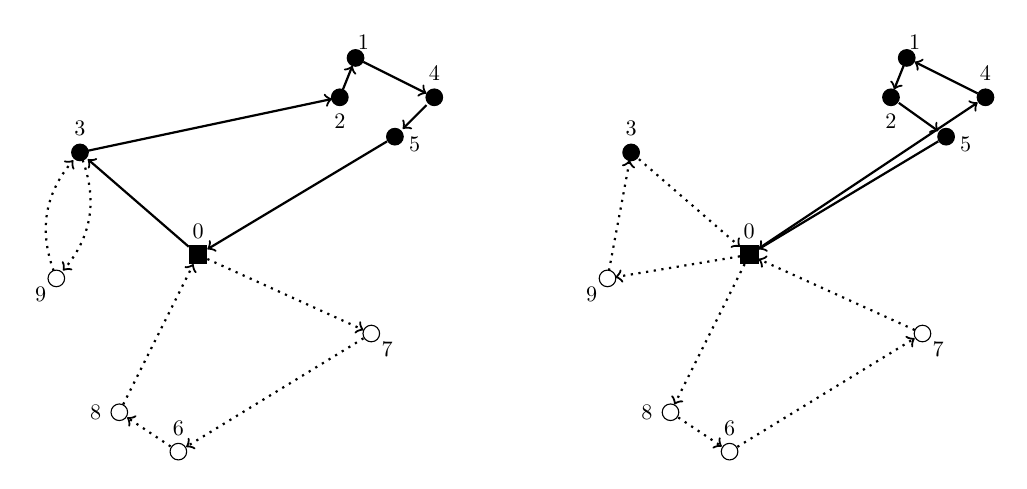
\begin{tikzpicture}[scale=1, every node/.style={scale=0.8}]
    
      % Depot
      \node[draw, fill=black, minimum size=8pt, shape=rectangle] (n0) at (0,0) {};
      \node at (0,0.3) {0};
      
      \node (n1) at (2.0,2.5) {};
      \node at (2.1,2.7) {1};
      
      \node (n2) at (1.80,2.00) {};
      \node at (1.8,1.7) {2};
      
      \node (n3) at (-1.50,1.30) {};
      \node at (-1.50,1.60) {3};
      
      \node (n4) at (3.0,2.00) {};
      \node at (3.0,2.30) {4};
      
      \node (n5) at (2.50,1.50) {};
      \node at (2.75,1.40) {5};
      
      \node (n6) at (-0.25,-2.5) {};
      \node at (-0.25,-2.2) {6};
      
      \node (n7) at (2.2,-1) {};
      \node at (2.4,-1.2) {7};
      
      \node (n8) at (-1.00,-2.0) {};
      \node at (-1.30,-2.0) {8};
      
      \node (n9) at (-1.80,-0.30) {};
      \node at (-2,-0.5) {9};
      
    
      % Route 1
      \draw[thick,-to] (n0) -- (n3);
      \draw[thick,-to] (n3) -- (n2);
      \draw[thick,-to] (n2) -- (n1);
      \draw[thick,-to] (n1) -- (n4);
      \draw[thick,-to] (n4) -- (n5);
      \draw[thick,-to] (n5) -- (n0);
      \filldraw[black] (n1) circle (3pt);
      \filldraw[black] (n2) circle (3pt);
      \filldraw[fill=white,draw=black] (n8) circle (3pt);
      \filldraw[fill=white,draw=black] (n7) circle (3pt);
      \filldraw[fill=white,draw=black] (n9) circle (3pt);
      \filldraw[black] (n3) circle (3pt);
    
      % Route 2
      \draw[thick,dotted,-to] (n0) -- (n7);
      \draw[thick, dotted,-to] (n7) -- (n6);
      \draw[thick, dotted,-to] (n6) -- (n8);
      \draw[thick, dotted,-to] (n8) -- (n0);
      \filldraw[fill=white,draw=black] (n6) circle (3pt);
      \filldraw[black] (n5) circle (3pt);
      \filldraw[black] (n4) circle (3pt);

      \draw[thick,dotted,-to] (n3) to[bend left=30] (n9);
      \draw[thick,dotted,-to] (n9) to[bend left=30] (n3);

      \begin{scope}[xshift=7cm]
          \node[draw, fill=black, minimum size=8pt, shape=rectangle] (n0) at (0,0) {};
          \node at (0,0.3) {0};
          
          \node (n1) at (2.0,2.5) {};
          \node at (2.1,2.7) {1};
          
          \node (n2) at (1.80,2.00) {};
          \node at (1.8,1.7) {2};
          
          \node (n3) at (-1.50,1.30) {};
          \node at (-1.50,1.60) {3};
          
          \node (n4) at (3.0,2.00) {};
          \node at (3.0,2.30) {4};
          
          \node (n5) at (2.50,1.50) {};
          \node at (2.75,1.40) {5};
          
          \node (n6) at (-0.25,-2.5) {};
          \node at (-0.25,-2.2) {6};
          
          \node (n7) at (2.2,-1) {};
          \node at (2.4,-1.2) {7};
          
          \node (n8) at (-1.00,-2.0) {};
          \node at (-1.30,-2.0) {8};
          
          \node (n9) at (-1.80,-0.30) {};
          \node at (-2,-0.5) {9};
          
        
          % Route 1
          \draw[thick,-to] (n0) -- (n4);
          \draw[thick,-to] (n4) -- (n1);
          \draw[thick,-to] (n1) -- (n2);
          \draw[thick,-to] (n2) -- (n5);
          \draw[thick,-to] (n5) -- (n0);
          \filldraw[black] (n1) circle (3pt);
          \filldraw[black] (n2) circle (3pt);
          \filldraw[fill=white,draw=black] (n8) circle (3pt);
          \filldraw[fill=white,draw=black] (n7) circle (3pt);
          \filldraw[fill=white,draw=black] (n9) circle (3pt);
          \filldraw[black] (n3) circle (3pt);
        
          % Route 2
          \draw[thick,dotted,-to] (n0) -- (n8);
          \draw[thick, dotted,-to] (n8) -- (n6);
          \draw[thick, dotted,-to] (n6) -- (n7);
          \draw[thick, dotted,-to] (n7) -- (n0);
          \filldraw[fill=white,draw=black] (n6) circle (3pt);
          \filldraw[black] (n5) circle (3pt);
          \filldraw[black] (n4) circle (3pt);
    
          \draw[thick,dotted,-to] (n0) -- (n9);
          \draw[thick,dotted,-to] (n9) -- (n3);
          \draw[thick,dotted,-to] (n3) -- (n0);
      \end{scope}
    
      % Legend
      % \begin{scope}[xshift=4cm, yshift=-0cm]
      %     \draw[fill=black] (0.15,0) rectangle +(0.2,0.2);
      %     \node[right=0.3cm] at (0.6,0.1) {Depósito};
      %     \filldraw[black] (0.25,-0.5) circle (3pt);
      %     \node[right=0.3cm] at (0.6,-0.5) {VC};
      %     \draw[black] (0.25,-1.1) circle (3pt);
      %     \node[right=0.3cm] at (0.6,-1.1) {TC};
      %     \draw[thick] (0,-1.6) -- (0.5,-1.6);
      %     \node[right=0.3cm] at (0.6,-1.6) {Ruta de vehículo};
      %     \draw[thick,dotted] (0,-2.1) -- (0.5,-2.1);
      %     \node[right=0.3cm] at (0.6,-2.1) {Ruta de camión};

          
      %   \end{scope}
    
    \end{tikzpicture}

    \caption{Comparación de la solución dada por Gurobi (\textit{izquierda)} para el problema P5 con la obtenida mediante el algoritmo memético (\textit{derecha}).}
    \label{fig:P5}
\end{figure}

Si ahora comparamos la solución dada por Gurobi para el problema P8 con la obtenida a partir del algoritmo memético (Figura \ref{fig:P8}), vemos que se obtiene la misma ruta, aunque en alguna ejecución, alguna de las rutas que compone la solución se encuentra invertida. Lo que indica esto es que el algoritmo funciona de manera correcta para aquellos problemas en cuya solución óptima no incluya una subruta que contenga clientes VC.  

\begin{figure}[H]
    \centering
    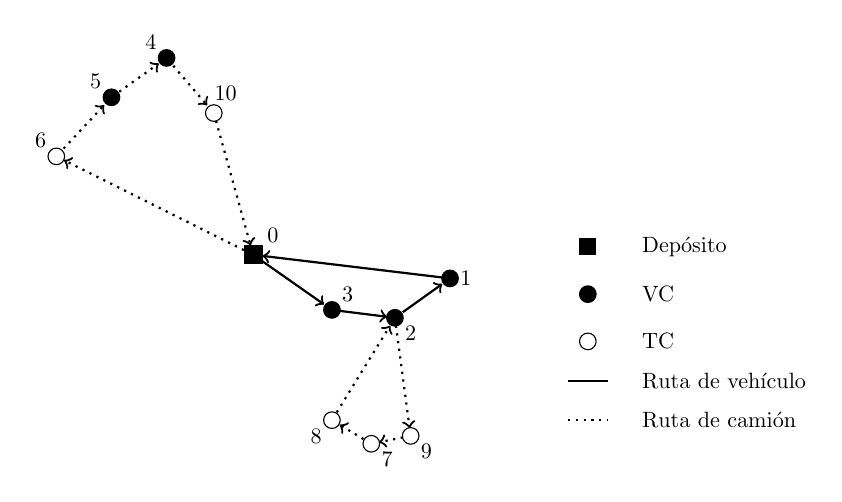
\begin{tikzpicture}[scale=1, every node/.style={scale=0.8}]
    
      % Depot
      \node[draw, fill=black, minimum size=8pt, shape=rectangle] (n0) at (0,0) {};
      \node at (0.25,0.25) {0};
      
      \node (n1) at (2.50,-0.30) {};
      \node at (2.7,-0.3) {1};
      
      \node (n2) at (1.80,-0.80) {};
      \node at (2.0,-1.0) {2};
      
      \node (n3) at (1.00,-0.70) {};
      \node at (1.2,-0.5) {3};
      
      \node (n4) at (-1.10,2.50) {};
      \node at (-1.3,2.7) {4};
      
      \node (n5) at (-1.80,2.00) {};
      \node at (-2.0,2.2) {5};
      
      \node (n6) at (-2.50,1.25) {};
      \node at (-2.7,1.45) {6};
      
      \node (n7) at (1.50,-2.40) {};
      \node at (1.7,-2.6) {7};
      
      \node (n8) at (1.00,-2.10) {};
      \node at (0.8,-2.3) {8};
      
      \node (n9) at (2.00,-2.30) {};
      \node at (2.2,-2.5) {9};
      
      \node (n10) at (-0.50,1.80) {};
      \node at (-0.35,2.05) {10};
    
      % Route 1
      \draw[thick,-to] (n0) -- (n3);
      \draw[thick,-to] (n3) -- (n2);
      \draw[thick, dotted,-to] (n2) -- (n9);
      \draw[thick, dotted,-to] (n9) -- (n7);
      \draw[thick, dotted,-to] (n7) -- (n8);
      \draw[thick, dotted,-to] (n8) -- (n2);
      \draw[thick,-to] (n2) -- (n1);
      \draw[thick,-to] (n1) -- (n0);
      \filldraw[black] (n1) circle (3pt);
      \filldraw[black] (n2) circle (3pt);
      \filldraw[fill=white,draw=black] (n8) circle (3pt);
      \filldraw[fill=white,draw=black] (n7) circle (3pt);
      \filldraw[fill=white,draw=black] (n9) circle (3pt);
      \filldraw[black] (n3) circle (3pt);
    
      % Route 2
      \draw[thick,dotted,-to] (n0) -- (n6);
      \draw[thick, dotted,-to] (n6) -- (n5);
      \draw[thick, dotted,-to] (n5) -- (n4);
      \draw[thick, dotted,-to] (n4) -- (n10);
      \draw[thick, dotted,-to] (n10) -- (n0);
      \filldraw[fill=white,draw=black] (n6) circle (3pt);
      \filldraw[black] (n5) circle (3pt);
      \filldraw[black] (n4) circle (3pt);
      \filldraw[fill=white,draw=black] (n10) circle (3pt);
    
      % Legend
      \begin{scope}[xshift=4cm, yshift=-0cm]
          \draw[fill=black] (0.15,0) rectangle +(0.2,0.2);
          \node[right=0.3cm] at (0.6,0.1) {Depósito};
          \filldraw[black] (0.25,-0.5) circle (3pt);
          \node[right=0.3cm] at (0.6,-0.5) {VC};
          \draw[black] (0.25,-1.1) circle (3pt);
          \node[right=0.3cm] at (0.6,-1.1) {TC};
          \draw[thick] (0,-1.6) -- (0.5,-1.6);
          \node[right=0.3cm] at (0.6,-1.6) {Ruta de vehículo};
          \draw[thick,dotted] (0,-2.1) -- (0.5,-2.1);
          \node[right=0.3cm] at (0.6,-2.1) {Ruta de camión};

          
        \end{scope}
    
    \end{tikzpicture}

    \caption{Esquema de la solución dada por el algoritmo MA para el problema P8. La solución es la misma para el problema resuelto por el método exacto Gurobi \cite{laura-mcttrp}.}
    \label{fig:P8}
\end{figure}
